\chapter{Oscilloscopio}
L'\textbf{oscilloscopio} svolge diversi compiti:
\begin{itemize}
    \item \textbf{Acquisire} (campionare  e quantizzare) un segnale
    \item \textbf{Visualizzare} un segnale
    \item \textbf{Misurare}
    \begin{itemize}
        \item Ampiezze
        \item Dominio del tempo
    \end{itemize}
\end{itemize}
Oltre a \textbf{rappresentare} il segnale, è in grado di verificare la presenza di \textbf{disturbi} nel segnare.\\
D'altra parte \textbf{si perde in termini di accuracy}, tuttavia posso lavorare a \textbf{frequenze alte} (10 GHz).
\section{Schema a Blocchi}
\begin{center}
    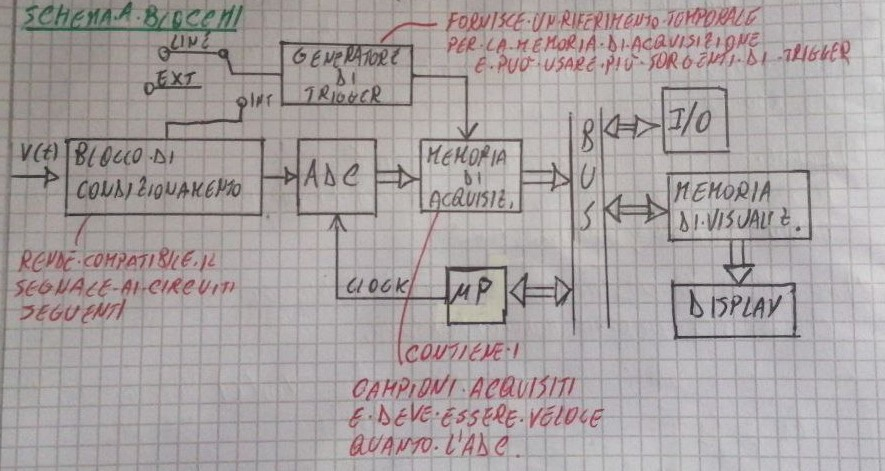
\includegraphics[width=\textwidth]{Images/figure14.jpg}
\end{center}
\section{Blocco di Condizionamento}
\begin{center}
    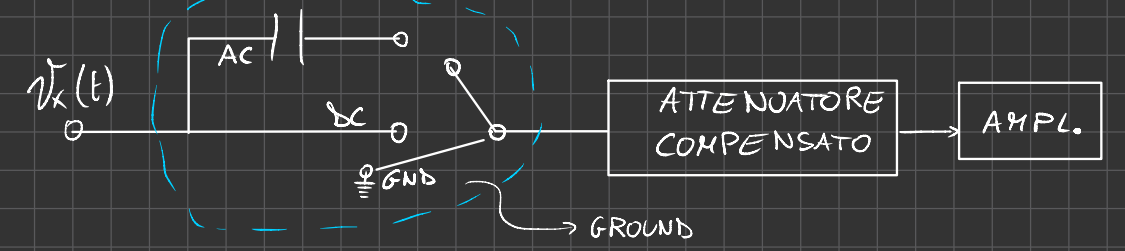
\includegraphics[width=\textwidth]{Images/figure15.png}
\end{center}
\subsection{Accoppiamento}
\begin{itemize}
    \item \textbf{DC}: Non altera il segnale
    \item \textbf{AC}: Passa prima per un condensatore serie che \textbf{filtra} ed \textbf{elimina} la \textbf{componente} \textbf{continua} (offset)
    \item \textbf{Ground}: Collega l'ingresso dell'oscilloscopio a \textbf{ground} per dargli delle condizioni iniziali di riferimento di potenza
\end{itemize}
\subsection{Att/Amp}
\begin{itemize}
    \item \textbf{Attenuatore}: \textbf{attenua} il segnale in accordo con il fondoscala dello strumento.
    \item \textbf{Amplificatore}: \textbf{amplifica} il segnale in accordo con il fondoscala dello strumento.
\end{itemize}
\subsection{Attenuatore Compensato}
\begin{center}
    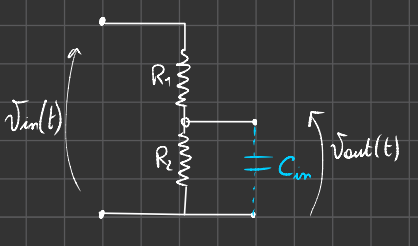
\includegraphics[width=.5\textwidth]{Images/figure16.png}
\end{center}
\begin{equation*}
    V_{out}(t) = V_{in}(t)  \frac{R_2}{R_1 + R_2}
\end{equation*}
\begin{equation*}
    C_{in} = \text{Capacità parassita piccola all'ingresso dell'amplificatore}
\end{equation*}
\begin{equation*}
    V_{out}(t) = V_{in}(t) \cdot \frac{(R_2 // C_{in})}{R_1 + (R_2 // C_{in})} = V_{in}(t)\cdot \frac{\frac{R_2}{j\w C_{in}}}{R_2 + \frac{1}{j\w C_{in}}} \cdot \frac{1}{R_1 + \frac{R_2}{\frac{j\w C_{in}}{R_2 + \frac{1}{j\w C_{in}}}}}
\end{equation*}
Dobbiamo \textbf{annullare} la \textbf{dipendenza} da $\w$ attraverso la \textbf{condizione di compensazione}:
\begin{itemize}
    \item Rendo \textbf{sistematico} ciò che è \textbf{aleatorio} (ovvero $C_{in}$):\\ 
    Metto in \textbf{parallelo} a $C_{in}$ una \textbf{capacità} $C_2$ di valore noto con un ordine di grandezza maggiore.
    \item ho ancora \textbf{dipendenza} da $\w$ quindi aggiungo un'altra \textbf{capacità} $C_1$ da scegliere in modo opportuno.
\end{itemize}
\begin{center}
    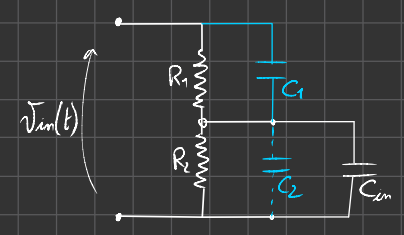
\includegraphics[width=.5\textwidth]{Images/figure17.png}
\end{center}
\begin{equation*}
    V_{out}(t) = \frac{Z_2}{Z_1 + Z_2} \cdot V_{in (t)} \ \text{deve essere indipendente da $\w$}
\end{equation*}
\begin{equation*}
    V_{out}(t) = \begin{dcases}
        \frac{R_2}{R_1 + R_2} V_{in}(t) \quad \w=0\\
        \frac{\frac{1}{j\w C_2}}{\frac{1}{j\w C_1} + \frac{1}{j\w C_2}} \cdot V_{in}(t) = \frac{ V_{in}(t)}{j\w C_2} \cdot \frac{-\w^2 C_1 C_2}{j\w C_1 + j\w C_2} \quad \w \longrightarrow \infty
    \end{dcases}
\end{equation*}
Quindi la \textbf{condizione di compensazione} è:
\begin{equation*}
    R_1 C_1 = R_2 C_2
\end{equation*}
\section{Generatore di Trigger}
Il \textbf{generatore di trigger} deve rispettare alcune esigenze:
\begin{itemize}
    \item Il punto in cui far partire la visualizzazione deve essere arbitrario
    \item La visualizzazione deve consentire di fare misure
\end{itemize}
Al suo interno troviamo:
\begin{center}
    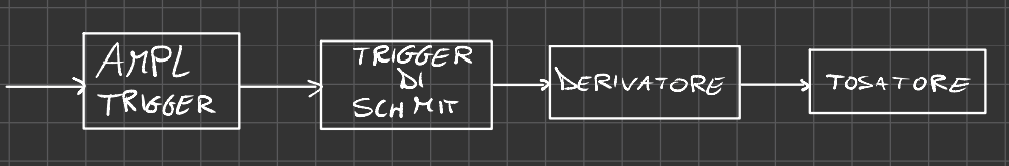
\includegraphics[width=.6\textwidth]{Images/figure18.png}
\end{center}
\section{Memoria di Acquisizione}
La \textbf{memoria} \textbf{di} \textbf{acquisizione} \textbf{circolare} usa una tecnica di memorizzazione \textbf{FIFO}:
\begin{center}
    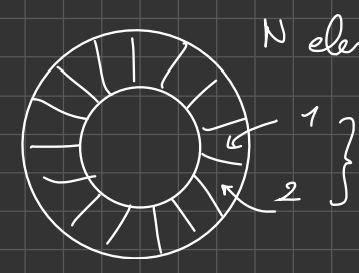
\includegraphics[width=.5\textwidth]{Images/figure19.png}
\end{center}
Esistono due modalità di memorizzazione:
\begin{itemize}
    \item \textbf{Tempo reale }
    \item \textbf{Tempo Equivalente}
    \begin{itemize}
        \item \textbf{Sincorno}
        \item \textbf{Asincrono}
    \end{itemize}
\end{itemize}
\subsection{Tempo Equivalente Sincrono}
Con segnali \textbf{periodici} è possibile evitare di soddisfare \textbf{Nyquist}:
\begin{center}
    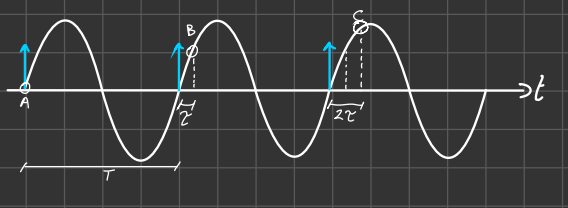
\includegraphics[width=.6\textwidth]{Images/figure20.png}
\end{center}
Dove $\tau = T_c = \left(1 + \frac{1}{M}\right)$.\\
\textbf{In pratica prendiamo un punto per periodo.}
\subsection{Tempo Equivalente Asincrono}
Il campione viene preso in modo \textbf{asincrono} rispetto al \textbf{trigger}
\begin{center}
    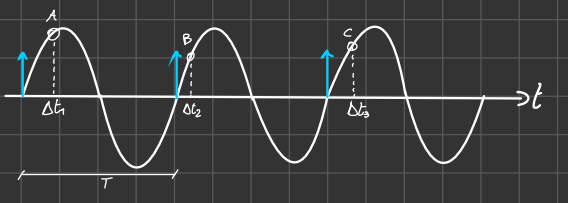
\includegraphics[width=.6\textwidth]{Images/figure21.png}
\end{center}
con $\Delta T_i$ diversi.\\
\textbf{Prendiamo un punto ogni periodo ma a diverse distanze dall'impulso di trigger.
}\section{Display}
\begin{center}
    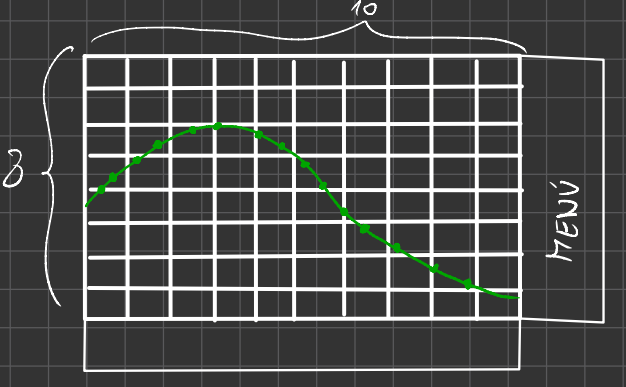
\includegraphics[width=.6\textwidth]{Images/figure22.png}
\end{center}
Attraverso il \textbf{display} è possibile fare alcune \textbf{misurazioni} grazie alle \textbf{griglie} che si trovano sovrapposte al segnale.\\ \\
Un'importante caratteristica di questo \textbf{display}, risiede nel fatto che un classico "\textbf{zoom}" corrisponde ad una diversa \textbf{attribuzione} di \textbf{tempo} o \textbf{tensione} alla \textbf{linea di griglia unitaria.}